%Chapter 4
\chapter{Results and validation}
\thispagestyle{empty}
\vspace{38em}
\hrulefill
\\
\enquote*{\textit{Quote.}} - Somebody\\
\newpage
\section{Introduction}

\section{Case study: MineA \color{blue}(Beatrix 123)}
	\subsection{Preamble}
This section will discuss the implementation of the simulation on a second case study. Further, the result of various simulated scenarios will be discussed. Finally validation of the the simulated scenarios using actual measurable tests will be discussed.
\subsection{System investigation}
\begin{figure}[h!]
	\centering
	\fbox{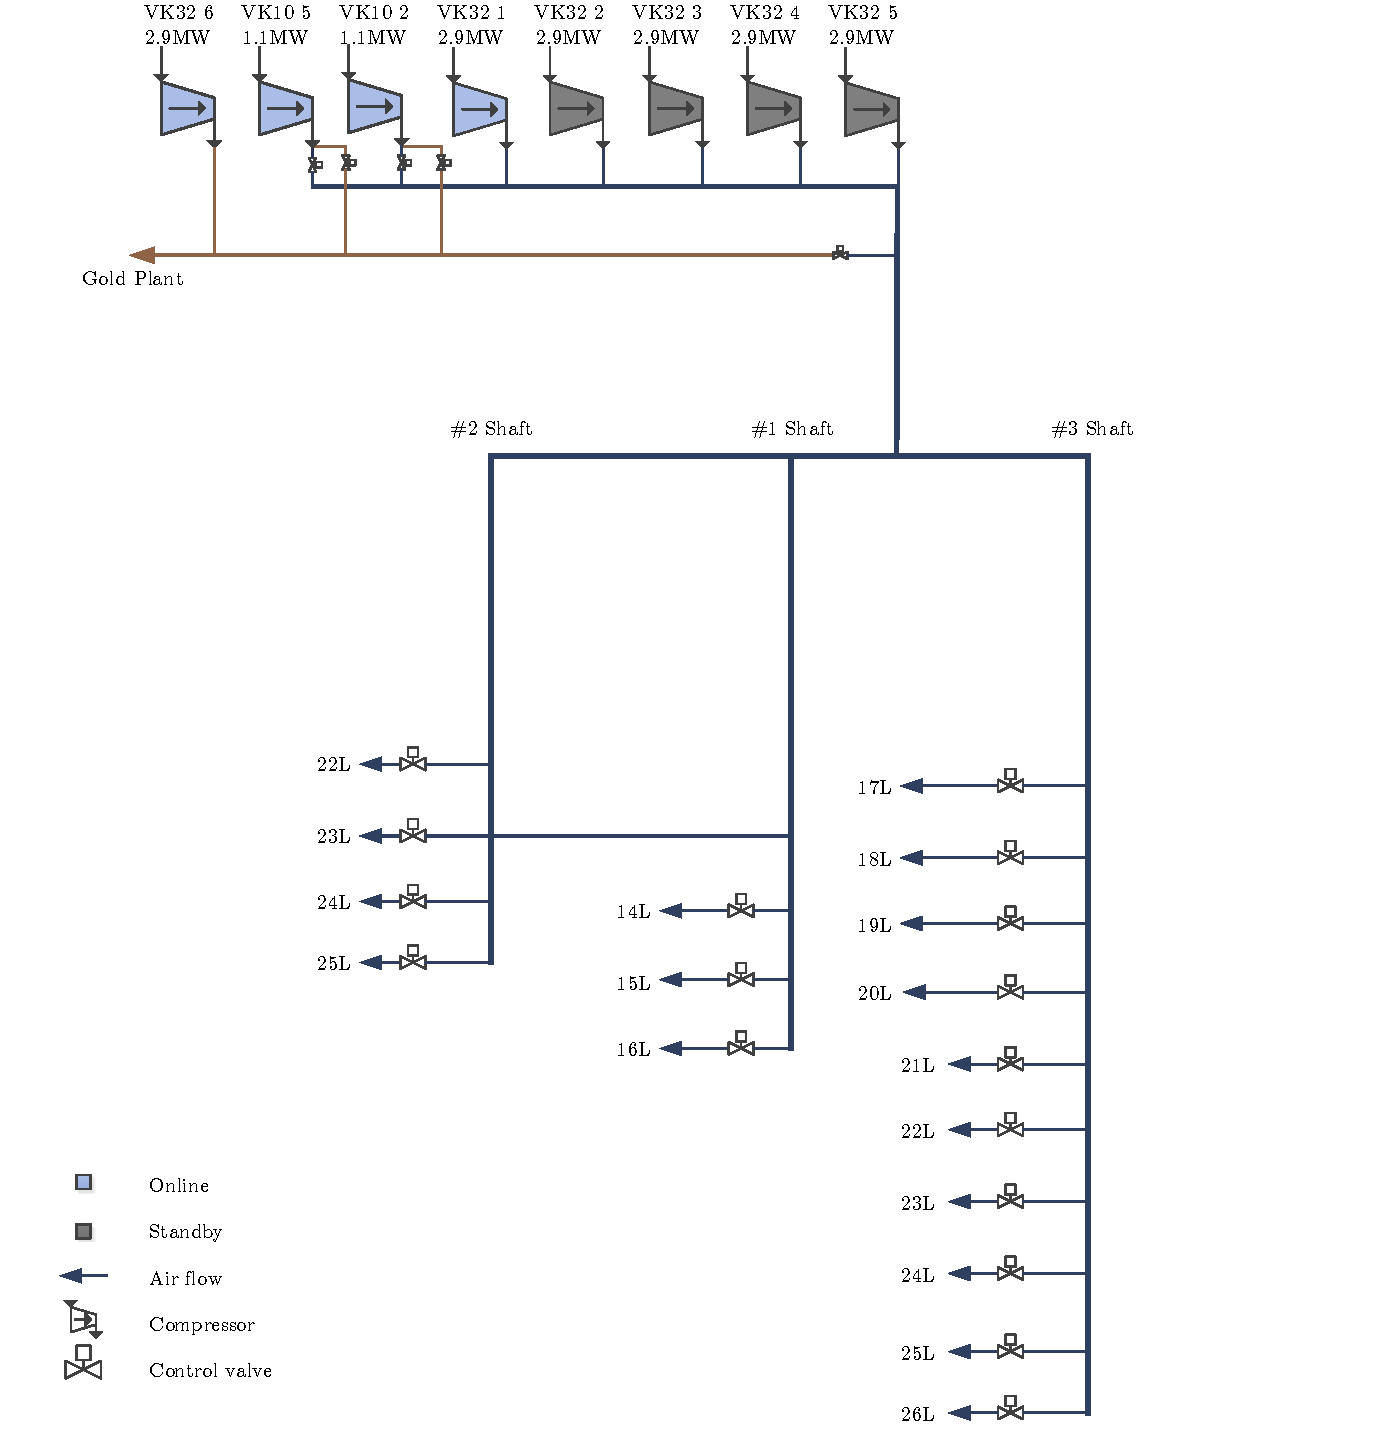
\includegraphics[trim =0cm 0.6cm 0cm 0.6cm,width=\textwidth]{Graphs/4/BeatLayout1/BeatLayout1.pdf}}
	\caption{Basic layout showing the distribution of the air network.}
	\label{fig: Beatrix Air layout}
\end{figure}
\subsection{Scenario 1. Compressor set points}
\subsection{Scenario 2. Control valves set points}
\subsection{Summary}
\newpage
\section{Case study: Mine B \color{blue}(Kusasalethu)}
	\subsection{Preamble}
	 This section will discuss the implementation of the simulation on a second case study. Further, the result of various simulated scenarios will be discussed. Finally validation of the the simulated scenarios using actual measurable tests will be discussed.
	\subsection{System investigation}
	The methodology was implemented on a large South African gold mine. The mine utilises five compressors supply compressed air to various surface and underground operations. An investigation was performed to gather the data and information required to build a simulation model of the network.
	\par 
	A basic air distribution layout was obtained, as shown in Figure \ref{fig: KUS Air layout}.  The more detailed layout in !!Appendix *!!,  indicates available meters and instrumentation as well as typical airflow splits to varios sections and levels of the mine.
	\par 
	
	\begin{figure}[h!]
		\centering
		\fbox{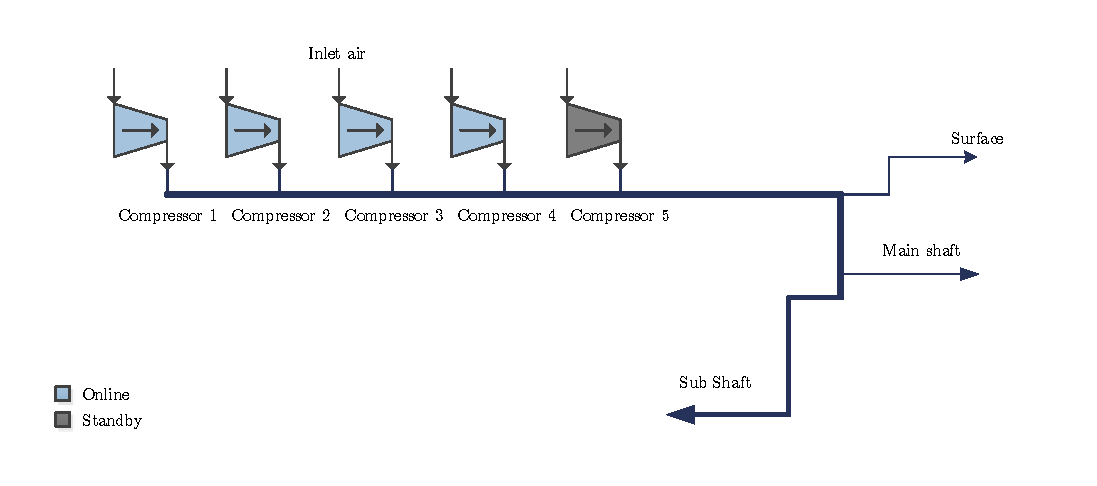
\includegraphics[trim =0cm 0.6cm 0cm 0.6cm,width=\textwidth]{Graphs/4/KUSLayout1/KUSLayout1.pdf}}
		\caption{Basic layout of the compressed air network.}
		\label{fig: KUS Air layout}
	\end{figure}
 To understand the operation of the system, schedules and setpoints as well as critical limits such as minimum and maximum pressures were obtained from various personal and from the \gls{scada}. Important data parameters such as Powers, pressures, flows, etc. for the system was gathered from the \gls{scada} and other data sources. This data will be used to develop and calibrate the simulation model
\par 
		
	An in-depth investigation was performed on the significant mining levels to map the locations of mining cross-sections, refuge bays, major leaks and other compressed air consumers on each level as well as measure the usages. An example of a resultant schematic from the underground investigation is shown in Figure \ref{fig: KUS Underground level layout}
	
	\begin{figure}[h!]
		\centering
		\fbox{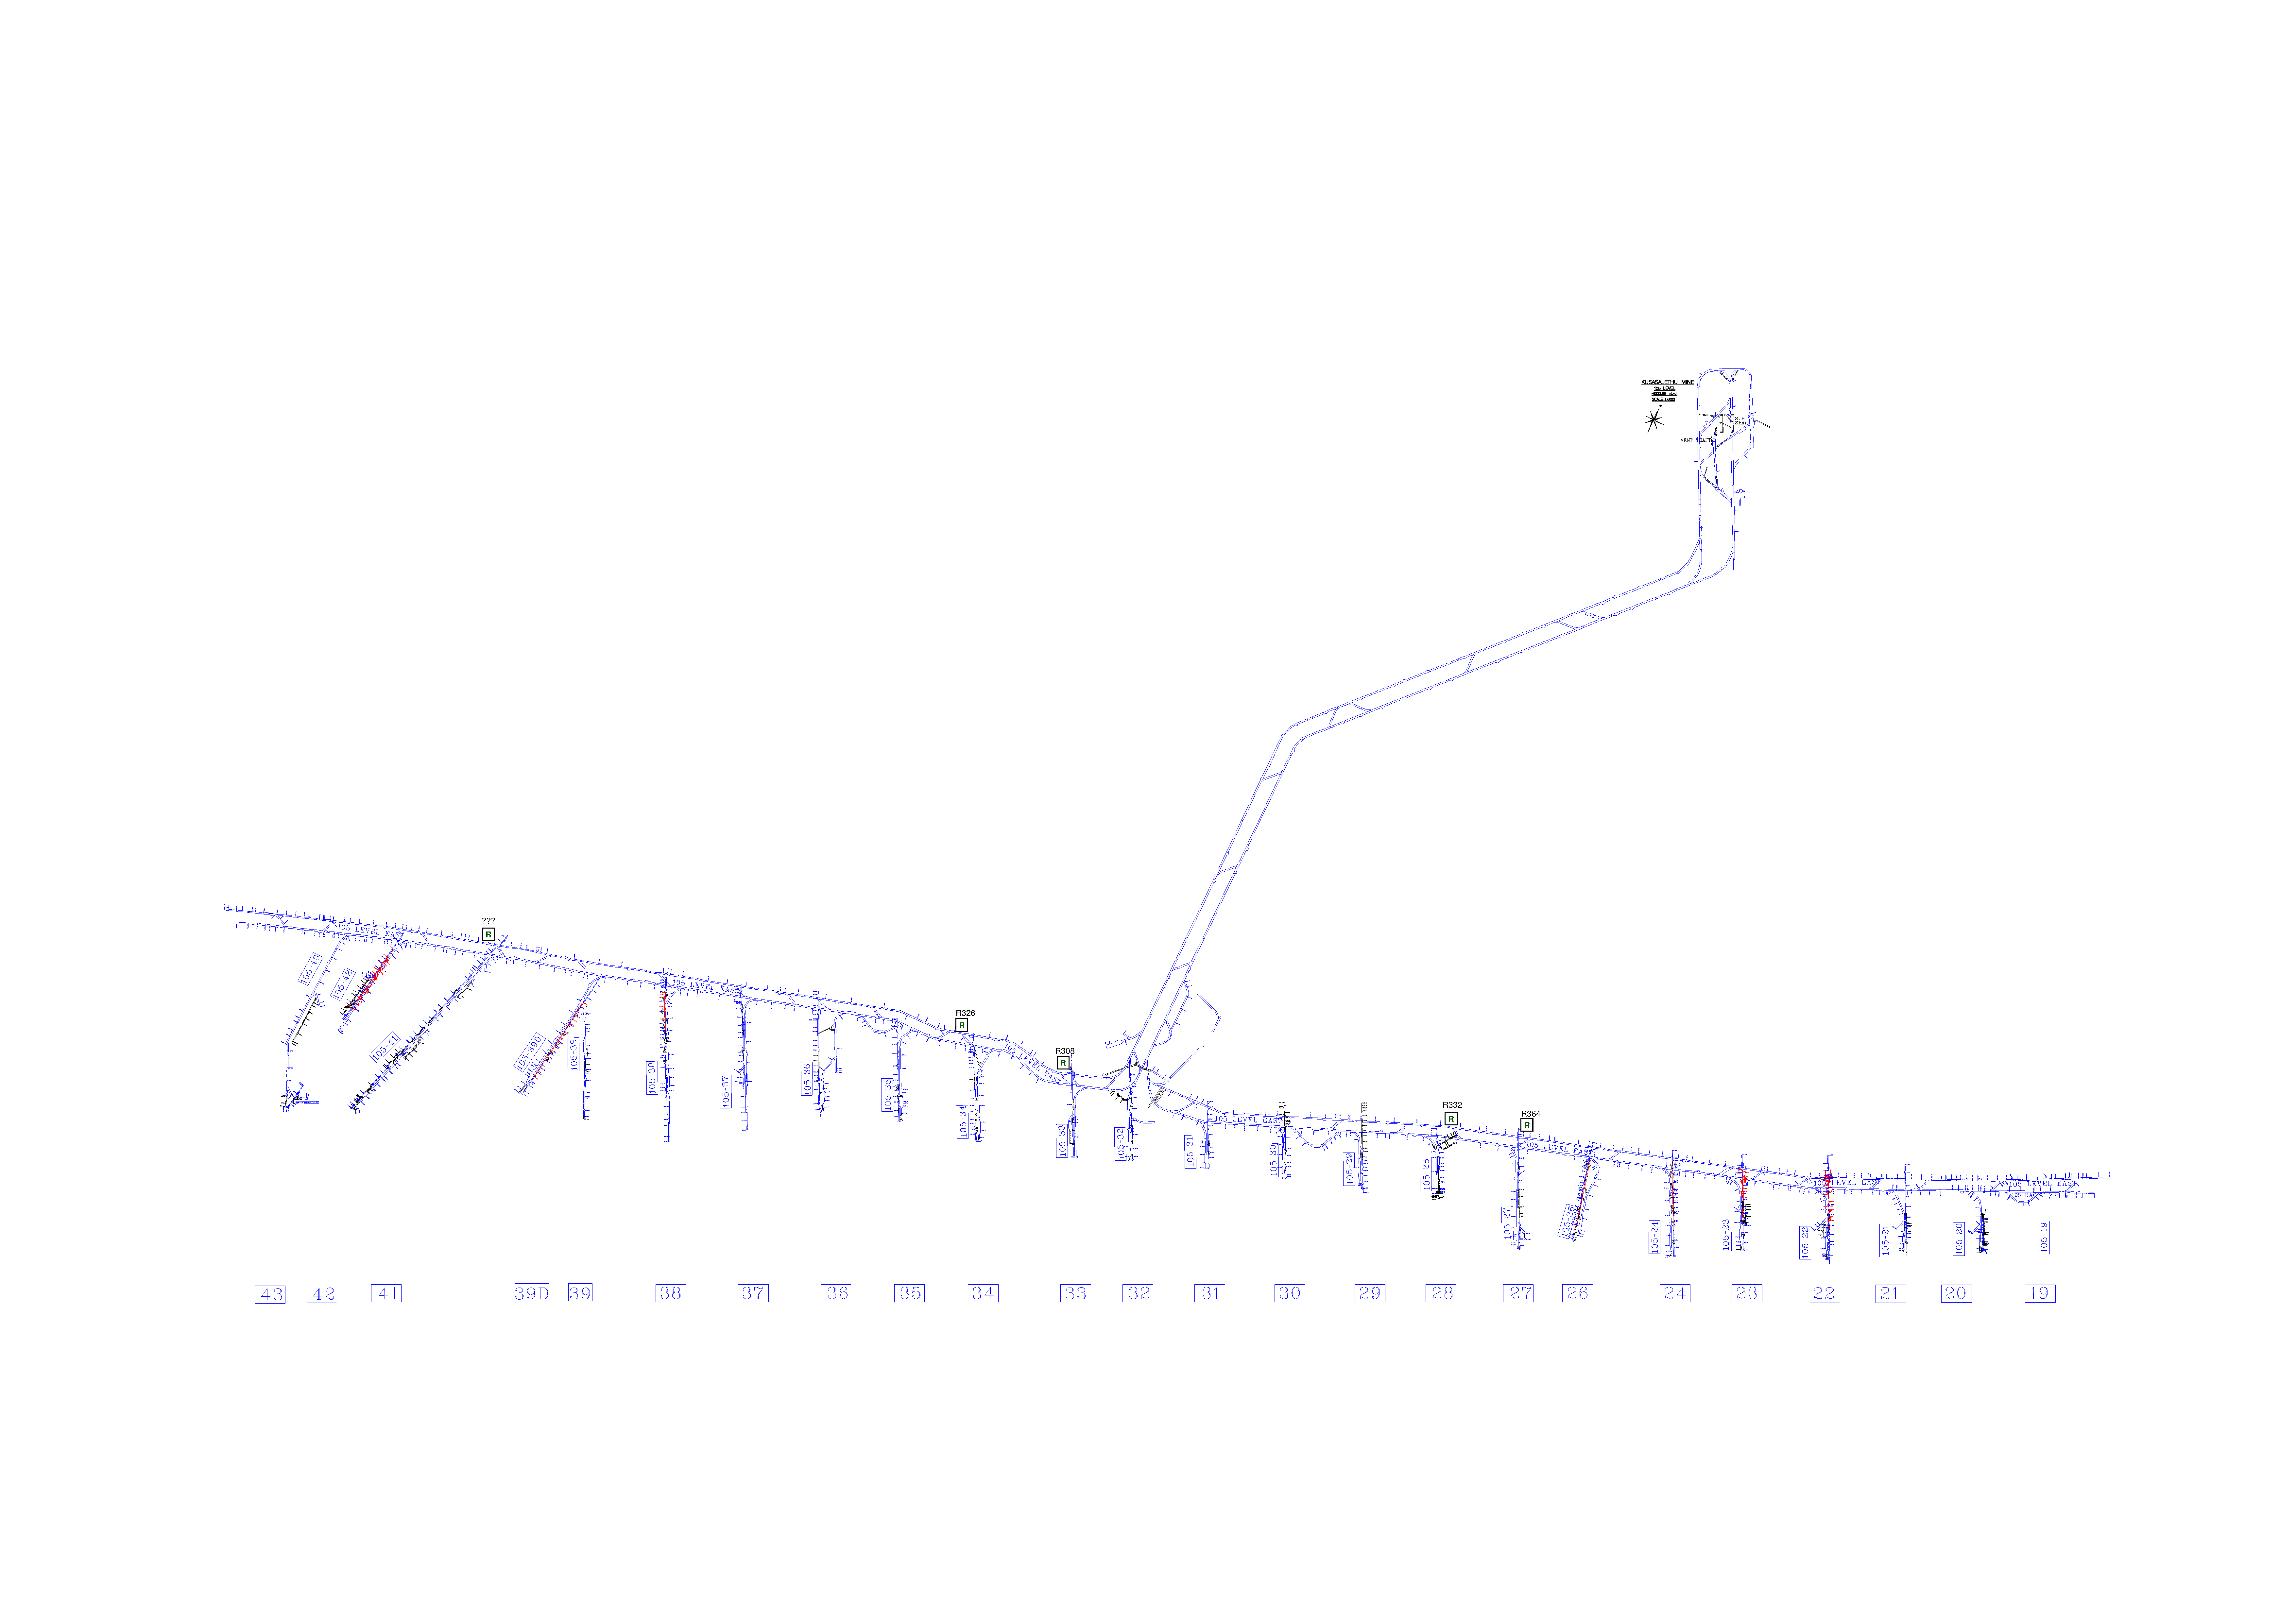
\includegraphics[trim =10cm 20cm 10cm 40cm, clip=true, width=\textwidth]{Graphs/4/LevelLayout/105L.pdf}}
		\caption{Underground level layout.}
		\label{fig: KUS Underground level layout}
	\end{figure}	
	\subsection{Model development}
	
	Using the data obtained from the investigation of the system, a  simulation model was developed in software. The modelling methodology described in Chapter 3 was then utilised to develop a model for the system. The entire model is shown in Appendix \ref{ASchematics} Figure \ref{fig: KUS Baseline model}. The model parameters were then calibrated to match the actual data from the mine.
	
	\subsubsection{Verification of baseline simulation}
	Verification of the model was performed firstly by comparing the simulation outputs to actual measured values. To simplify the model, the actual measured pressure is temporarily used as set points for the compressors. This ensured that the pressure in the network is identical to that of the actual measured system as shown in Figure \ref{fig: Verification Pressure kusasalethu}.
	\par 
	
	\begin{figure}[h]
		\centering
		\fbox{% GNUPLOT: LaTeX picture with Postscript
\begingroup
  \makeatletter
  \providecommand\color[2][]{%
    \GenericError{(gnuplot) \space\space\space\@spaces}{%
      Package color not loaded in conjunction with
      terminal option `colourtext'%
    }{See the gnuplot documentation for explanation.%
    }{Either use 'blacktext' in gnuplot or load the package
      color.sty in LaTeX.}%
    \renewcommand\color[2][]{}%
  }%
  \providecommand\includegraphics[2][]{%
    \GenericError{(gnuplot) \space\space\space\@spaces}{%
      Package graphicx or graphics not loaded%
    }{See the gnuplot documentation for explanation.%
    }{The gnuplot epslatex terminal needs graphicx.sty or graphics.sty.}%
    \renewcommand\includegraphics[2][]{}%
  }%
  \providecommand\rotatebox[2]{#2}%
  \@ifundefined{ifGPcolor}{%
    \newif\ifGPcolor
    \GPcolortrue
  }{}%
  \@ifundefined{ifGPblacktext}{%
    \newif\ifGPblacktext
    \GPblacktextfalse
  }{}%
  % define a \g@addto@macro without @ in the name:
  \let\gplgaddtomacro\g@addto@macro
  % define empty templates for all commands taking text:
  \gdef\gplbacktext{}%
  \gdef\gplfronttext{}%
  \makeatother
  \ifGPblacktext
    % no textcolor at all
    \def\colorrgb#1{}%
    \def\colorgray#1{}%
  \else
    % gray or color?
    \ifGPcolor
      \def\colorrgb#1{\color[rgb]{#1}}%
      \def\colorgray#1{\color[gray]{#1}}%
      \expandafter\def\csname LTw\endcsname{\color{white}}%
      \expandafter\def\csname LTb\endcsname{\color{black}}%
      \expandafter\def\csname LTa\endcsname{\color{black}}%
      \expandafter\def\csname LT0\endcsname{\color[rgb]{1,0,0}}%
      \expandafter\def\csname LT1\endcsname{\color[rgb]{0,1,0}}%
      \expandafter\def\csname LT2\endcsname{\color[rgb]{0,0,1}}%
      \expandafter\def\csname LT3\endcsname{\color[rgb]{1,0,1}}%
      \expandafter\def\csname LT4\endcsname{\color[rgb]{0,1,1}}%
      \expandafter\def\csname LT5\endcsname{\color[rgb]{1,1,0}}%
      \expandafter\def\csname LT6\endcsname{\color[rgb]{0,0,0}}%
      \expandafter\def\csname LT7\endcsname{\color[rgb]{1,0.3,0}}%
      \expandafter\def\csname LT8\endcsname{\color[rgb]{0.5,0.5,0.5}}%
    \else
      % gray
      \def\colorrgb#1{\color{black}}%
      \def\colorgray#1{\color[gray]{#1}}%
      \expandafter\def\csname LTw\endcsname{\color{white}}%
      \expandafter\def\csname LTb\endcsname{\color{black}}%
      \expandafter\def\csname LTa\endcsname{\color{black}}%
      \expandafter\def\csname LT0\endcsname{\color{black}}%
      \expandafter\def\csname LT1\endcsname{\color{black}}%
      \expandafter\def\csname LT2\endcsname{\color{black}}%
      \expandafter\def\csname LT3\endcsname{\color{black}}%
      \expandafter\def\csname LT4\endcsname{\color{black}}%
      \expandafter\def\csname LT5\endcsname{\color{black}}%
      \expandafter\def\csname LT6\endcsname{\color{black}}%
      \expandafter\def\csname LT7\endcsname{\color{black}}%
      \expandafter\def\csname LT8\endcsname{\color{black}}%
    \fi
  \fi
    \setlength{\unitlength}{0.0500bp}%
    \ifx\gptboxheight\undefined%
      \newlength{\gptboxheight}%
      \newlength{\gptboxwidth}%
      \newsavebox{\gptboxtext}%
    \fi%
    \setlength{\fboxrule}{0.5pt}%
    \setlength{\fboxsep}{1pt}%
\begin{picture}(9360.00,2772.00)%
    \gplgaddtomacro\gplbacktext{%
      \colorrgb{0.00,0.00,0.00}%
      \put(814,924){\makebox(0,0)[r]{\strut{}$300$}}%
      \colorrgb{0.00,0.00,0.00}%
      \put(814,1452){\makebox(0,0)[r]{\strut{}$350$}}%
      \colorrgb{0.00,0.00,0.00}%
      \put(814,1979){\makebox(0,0)[r]{\strut{}$400$}}%
      \colorrgb{0.00,0.00,0.00}%
      \put(814,2507){\makebox(0,0)[r]{\strut{}$450$}}%
      \colorrgb{0.00,0.00,0.00}%
      \put(946,704){\makebox(0,0){\strut{}00:00}}%
      \colorrgb{0.00,0.00,0.00}%
      \put(2157,704){\makebox(0,0){\strut{}04:00}}%
      \colorrgb{0.00,0.00,0.00}%
      \put(3369,704){\makebox(0,0){\strut{}08:00}}%
      \colorrgb{0.00,0.00,0.00}%
      \put(4580,704){\makebox(0,0){\strut{}12:00}}%
      \colorrgb{0.00,0.00,0.00}%
      \put(5791,704){\makebox(0,0){\strut{}16:00}}%
      \colorrgb{0.00,0.00,0.00}%
      \put(7003,704){\makebox(0,0){\strut{}20:00}}%
      \colorrgb{0.00,0.00,0.00}%
      \put(8214,704){\makebox(0,0){\strut{}00:00}}%
      \colorrgb{0.00,0.00,0.00}%
      \put(8346,924){\makebox(0,0)[l]{\strut{}$0$}}%
      \colorrgb{0.00,0.00,0.00}%
      \put(8346,1557){\makebox(0,0)[l]{\strut{}$10$}}%
      \colorrgb{0.00,0.00,0.00}%
      \put(8346,2190){\makebox(0,0)[l]{\strut{}$20$}}%
    }%
    \gplgaddtomacro\gplfronttext{%
      \csname LTb\endcsname%
      \put(176,1715){\rotatebox{-270}{\makebox(0,0){\strut{}Pressure $(kPa)$}}}%
      \put(8851,1715){\rotatebox{-270}{\makebox(0,0){\strut{}$\% error$}}}%
      \put(4580,374){\makebox(0,0){\strut{}Time of Day}}%
      \csname LTb\endcsname%
      \put(2241,173){\makebox(0,0)[r]{\strut{}Baseline press.}}%
      \csname LTb\endcsname%
      \put(5208,173){\makebox(0,0)[r]{\strut{}Simulated press.}}%
      \csname LTb\endcsname%
      \put(8175,173){\makebox(0,0)[r]{\strut{}Error}}%
    }%
    \gplbacktext
    \put(0,0){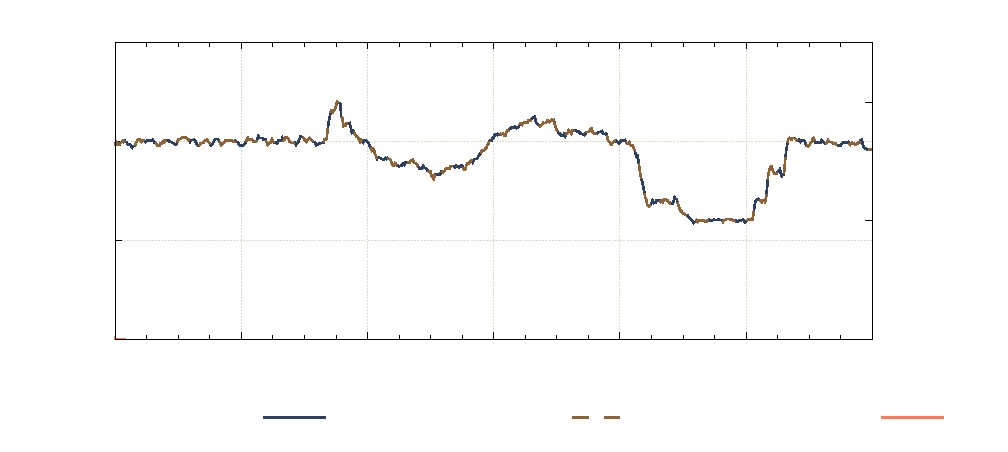
\includegraphics{Graphs/4/KusVerify/Pressure/Pressure}}%
    \gplfronttext
  \end{picture}%
\endgroup
}
		\caption{Comparing the pressure response of simulation compared to the actual measured pressure}
		\label{fig: Verification Pressure kusasalethu}
	\end{figure}

 	With the pressure set, the power and air flow outputs for components throughout the model were compared with their relative actual values. Figure \ref{fig: Verification Power kusasalethu} shows the comparison of the total power and flow of the system with the actual measure values for that same period. The accuracy for these parameters compared to the real system was $98.7 \%$ and $99.0 \%$ respectively. This was regarded as acceptable accuracy. 
 
	\begin{figure}[h]
		\centering
		\fbox{% GNUPLOT: LaTeX picture with Postscript
\begingroup
  \makeatletter
  \providecommand\color[2][]{%
    \GenericError{(gnuplot) \space\space\space\@spaces}{%
      Package color not loaded in conjunction with
      terminal option `colourtext'%
    }{See the gnuplot documentation for explanation.%
    }{Either use 'blacktext' in gnuplot or load the package
      color.sty in LaTeX.}%
    \renewcommand\color[2][]{}%
  }%
  \providecommand\includegraphics[2][]{%
    \GenericError{(gnuplot) \space\space\space\@spaces}{%
      Package graphicx or graphics not loaded%
    }{See the gnuplot documentation for explanation.%
    }{The gnuplot epslatex terminal needs graphicx.sty or graphics.sty.}%
    \renewcommand\includegraphics[2][]{}%
  }%
  \providecommand\rotatebox[2]{#2}%
  \@ifundefined{ifGPcolor}{%
    \newif\ifGPcolor
    \GPcolortrue
  }{}%
  \@ifundefined{ifGPblacktext}{%
    \newif\ifGPblacktext
    \GPblacktextfalse
  }{}%
  % define a \g@addto@macro without @ in the name:
  \let\gplgaddtomacro\g@addto@macro
  % define empty templates for all commands taking text:
  \gdef\gplbacktext{}%
  \gdef\gplfronttext{}%
  \makeatother
  \ifGPblacktext
    % no textcolor at all
    \def\colorrgb#1{}%
    \def\colorgray#1{}%
  \else
    % gray or color?
    \ifGPcolor
      \def\colorrgb#1{\color[rgb]{#1}}%
      \def\colorgray#1{\color[gray]{#1}}%
      \expandafter\def\csname LTw\endcsname{\color{white}}%
      \expandafter\def\csname LTb\endcsname{\color{black}}%
      \expandafter\def\csname LTa\endcsname{\color{black}}%
      \expandafter\def\csname LT0\endcsname{\color[rgb]{1,0,0}}%
      \expandafter\def\csname LT1\endcsname{\color[rgb]{0,1,0}}%
      \expandafter\def\csname LT2\endcsname{\color[rgb]{0,0,1}}%
      \expandafter\def\csname LT3\endcsname{\color[rgb]{1,0,1}}%
      \expandafter\def\csname LT4\endcsname{\color[rgb]{0,1,1}}%
      \expandafter\def\csname LT5\endcsname{\color[rgb]{1,1,0}}%
      \expandafter\def\csname LT6\endcsname{\color[rgb]{0,0,0}}%
      \expandafter\def\csname LT7\endcsname{\color[rgb]{1,0.3,0}}%
      \expandafter\def\csname LT8\endcsname{\color[rgb]{0.5,0.5,0.5}}%
    \else
      % gray
      \def\colorrgb#1{\color{black}}%
      \def\colorgray#1{\color[gray]{#1}}%
      \expandafter\def\csname LTw\endcsname{\color{white}}%
      \expandafter\def\csname LTb\endcsname{\color{black}}%
      \expandafter\def\csname LTa\endcsname{\color{black}}%
      \expandafter\def\csname LT0\endcsname{\color{black}}%
      \expandafter\def\csname LT1\endcsname{\color{black}}%
      \expandafter\def\csname LT2\endcsname{\color{black}}%
      \expandafter\def\csname LT3\endcsname{\color{black}}%
      \expandafter\def\csname LT4\endcsname{\color{black}}%
      \expandafter\def\csname LT5\endcsname{\color{black}}%
      \expandafter\def\csname LT6\endcsname{\color{black}}%
      \expandafter\def\csname LT7\endcsname{\color{black}}%
      \expandafter\def\csname LT8\endcsname{\color{black}}%
    \fi
  \fi
    \setlength{\unitlength}{0.0500bp}%
    \ifx\gptboxheight\undefined%
      \newlength{\gptboxheight}%
      \newlength{\gptboxwidth}%
      \newsavebox{\gptboxtext}%
    \fi%
    \setlength{\fboxrule}{0.5pt}%
    \setlength{\fboxsep}{1pt}%
\begin{picture}(9360.00,3276.00)%
    \gplgaddtomacro\gplbacktext{%
      \colorrgb{0.00,0.00,0.00}%
      \put(682,924){\makebox(0,0)[r]{\strut{}$30$}}%
      \colorrgb{0.00,0.00,0.00}%
      \put(682,1967){\makebox(0,0)[r]{\strut{}$40$}}%
      \colorrgb{0.00,0.00,0.00}%
      \put(682,3011){\makebox(0,0)[r]{\strut{}$50$}}%
      \colorrgb{0.00,0.00,0.00}%
      \put(814,704){\makebox(0,0){\strut{}00:00}}%
      \colorrgb{0.00,0.00,0.00}%
      \put(2047,704){\makebox(0,0){\strut{}04:00}}%
      \colorrgb{0.00,0.00,0.00}%
      \put(3281,704){\makebox(0,0){\strut{}08:00}}%
      \colorrgb{0.00,0.00,0.00}%
      \put(4514,704){\makebox(0,0){\strut{}12:00}}%
      \colorrgb{0.00,0.00,0.00}%
      \put(5747,704){\makebox(0,0){\strut{}16:00}}%
      \colorrgb{0.00,0.00,0.00}%
      \put(6981,704){\makebox(0,0){\strut{}20:00}}%
      \colorrgb{0.00,0.00,0.00}%
      \put(8214,704){\makebox(0,0){\strut{}00:00}}%
      \colorrgb{0.00,0.00,0.00}%
      \put(8346,924){\makebox(0,0)[l]{\strut{}$0$}}%
      \colorrgb{0.00,0.00,0.00}%
      \put(8346,1759){\makebox(0,0)[l]{\strut{}$10$}}%
      \colorrgb{0.00,0.00,0.00}%
      \put(8346,2594){\makebox(0,0)[l]{\strut{}$20$}}%
    }%
    \gplgaddtomacro\gplfronttext{%
      \csname LTb\endcsname%
      \put(176,1967){\rotatebox{-270}{\makebox(0,0){\strut{}flow $(kg/s)$}}}%
      \put(8851,1967){\rotatebox{-270}{\makebox(0,0){\strut{}$\% error$}}}%
      \put(4514,374){\makebox(0,0){\strut{}Time of Day}}%
      \csname LTb\endcsname%
      \put(2307,173){\makebox(0,0)[r]{\strut{}Baseline flow}}%
      \csname LTb\endcsname%
      \put(5010,173){\makebox(0,0)[r]{\strut{}Simulated flow}}%
      \csname LTb\endcsname%
      \put(7713,173){\makebox(0,0)[r]{\strut{}Error}}%
    }%
    \gplbacktext
    \put(0,0){\fbox{
\includegraphics[trim=0 0 0.1cm 0, clip]{Graphs/4/KusVerify/Flow/Flow}}}%
    \gplfronttext
  \end{picture}%
\endgroup
}
		(a)\\
		\fbox{% GNUPLOT: LaTeX picture with Postscript
\begingroup
  \makeatletter
  \providecommand\color[2][]{%
    \GenericError{(gnuplot) \space\space\space\@spaces}{%
      Package color not loaded in conjunction with
      terminal option `colourtext'%
    }{See the gnuplot documentation for explanation.%
    }{Either use 'blacktext' in gnuplot or load the package
      color.sty in LaTeX.}%
    \renewcommand\color[2][]{}%
  }%
  \providecommand\includegraphics[2][]{%
    \GenericError{(gnuplot) \space\space\space\@spaces}{%
      Package graphicx or graphics not loaded%
    }{See the gnuplot documentation for explanation.%
    }{The gnuplot epslatex terminal needs graphicx.sty or graphics.sty.}%
    \renewcommand\includegraphics[2][]{}%
  }%
  \providecommand\rotatebox[2]{#2}%
  \@ifundefined{ifGPcolor}{%
    \newif\ifGPcolor
    \GPcolortrue
  }{}%
  \@ifundefined{ifGPblacktext}{%
    \newif\ifGPblacktext
    \GPblacktextfalse
  }{}%
  % define a \g@addto@macro without @ in the name:
  \let\gplgaddtomacro\g@addto@macro
  % define empty templates for all commands taking text:
  \gdef\gplbacktext{}%
  \gdef\gplfronttext{}%
  \makeatother
  \ifGPblacktext
    % no textcolor at all
    \def\colorrgb#1{}%
    \def\colorgray#1{}%
  \else
    % gray or color?
    \ifGPcolor
      \def\colorrgb#1{\color[rgb]{#1}}%
      \def\colorgray#1{\color[gray]{#1}}%
      \expandafter\def\csname LTw\endcsname{\color{white}}%
      \expandafter\def\csname LTb\endcsname{\color{black}}%
      \expandafter\def\csname LTa\endcsname{\color{black}}%
      \expandafter\def\csname LT0\endcsname{\color[rgb]{1,0,0}}%
      \expandafter\def\csname LT1\endcsname{\color[rgb]{0,1,0}}%
      \expandafter\def\csname LT2\endcsname{\color[rgb]{0,0,1}}%
      \expandafter\def\csname LT3\endcsname{\color[rgb]{1,0,1}}%
      \expandafter\def\csname LT4\endcsname{\color[rgb]{0,1,1}}%
      \expandafter\def\csname LT5\endcsname{\color[rgb]{1,1,0}}%
      \expandafter\def\csname LT6\endcsname{\color[rgb]{0,0,0}}%
      \expandafter\def\csname LT7\endcsname{\color[rgb]{1,0.3,0}}%
      \expandafter\def\csname LT8\endcsname{\color[rgb]{0.5,0.5,0.5}}%
    \else
      % gray
      \def\colorrgb#1{\color{black}}%
      \def\colorgray#1{\color[gray]{#1}}%
      \expandafter\def\csname LTw\endcsname{\color{white}}%
      \expandafter\def\csname LTb\endcsname{\color{black}}%
      \expandafter\def\csname LTa\endcsname{\color{black}}%
      \expandafter\def\csname LT0\endcsname{\color{black}}%
      \expandafter\def\csname LT1\endcsname{\color{black}}%
      \expandafter\def\csname LT2\endcsname{\color{black}}%
      \expandafter\def\csname LT3\endcsname{\color{black}}%
      \expandafter\def\csname LT4\endcsname{\color{black}}%
      \expandafter\def\csname LT5\endcsname{\color{black}}%
      \expandafter\def\csname LT6\endcsname{\color{black}}%
      \expandafter\def\csname LT7\endcsname{\color{black}}%
      \expandafter\def\csname LT8\endcsname{\color{black}}%
    \fi
  \fi
    \setlength{\unitlength}{0.0500bp}%
    \ifx\gptboxheight\undefined%
      \newlength{\gptboxheight}%
      \newlength{\gptboxwidth}%
      \newsavebox{\gptboxtext}%
    \fi%
    \setlength{\fboxrule}{0.5pt}%
    \setlength{\fboxsep}{1pt}%
\begin{picture}(9360.00,3276.00)%
    \gplgaddtomacro\gplbacktext{%
      \colorrgb{0.00,0.00,0.00}%
      \put(682,924){\makebox(0,0)[r]{\strut{}$8$}}%
      \colorrgb{0.00,0.00,0.00}%
      \put(682,1222){\makebox(0,0)[r]{\strut{}$9$}}%
      \colorrgb{0.00,0.00,0.00}%
      \put(682,1520){\makebox(0,0)[r]{\strut{}$10$}}%
      \colorrgb{0.00,0.00,0.00}%
      \put(682,1818){\makebox(0,0)[r]{\strut{}$11$}}%
      \colorrgb{0.00,0.00,0.00}%
      \put(682,2117){\makebox(0,0)[r]{\strut{}$12$}}%
      \colorrgb{0.00,0.00,0.00}%
      \put(682,2415){\makebox(0,0)[r]{\strut{}$13$}}%
      \colorrgb{0.00,0.00,0.00}%
      \put(682,2713){\makebox(0,0)[r]{\strut{}$14$}}%
      \colorrgb{0.00,0.00,0.00}%
      \put(682,3011){\makebox(0,0)[r]{\strut{}$15$}}%
      \colorrgb{0.00,0.00,0.00}%
      \put(814,704){\makebox(0,0){\strut{}00:00}}%
      \colorrgb{0.00,0.00,0.00}%
      \put(2047,704){\makebox(0,0){\strut{}04:00}}%
      \colorrgb{0.00,0.00,0.00}%
      \put(3281,704){\makebox(0,0){\strut{}08:00}}%
      \colorrgb{0.00,0.00,0.00}%
      \put(4514,704){\makebox(0,0){\strut{}12:00}}%
      \colorrgb{0.00,0.00,0.00}%
      \put(5747,704){\makebox(0,0){\strut{}16:00}}%
      \colorrgb{0.00,0.00,0.00}%
      \put(6981,704){\makebox(0,0){\strut{}20:00}}%
      \colorrgb{0.00,0.00,0.00}%
      \put(8214,704){\makebox(0,0){\strut{}00:00}}%
      \colorrgb{0.00,0.00,0.00}%
      \put(8346,924){\makebox(0,0)[l]{\strut{}$0$}}%
      \colorrgb{0.00,0.00,0.00}%
      \put(8346,1759){\makebox(0,0)[l]{\strut{}$10$}}%
      \colorrgb{0.00,0.00,0.00}%
      \put(8346,2594){\makebox(0,0)[l]{\strut{}$20$}}%
    }%
    \gplgaddtomacro\gplfronttext{%
      \csname LTb\endcsname%
      \put(176,1967){\rotatebox{-270}{\makebox(0,0){\strut{}Power $(MW)$}}}%
      \put(8851,1967){\rotatebox{-270}{\makebox(0,0){\strut{}$\% error$}}}%
      \put(4514,374){\makebox(0,0){\strut{}Time of Day}}%
      \csname LTb\endcsname%
      \put(2241,173){\makebox(0,0)[r]{\strut{}Baseline power}}%
      \csname LTb\endcsname%
      \put(5076,173){\makebox(0,0)[r]{\strut{}Simulated power}}%
      \csname LTb\endcsname%
      \put(7911,173){\makebox(0,0)[r]{\strut{}Error}}%
    }%
    \gplbacktext
    \put(0,0){\fbox{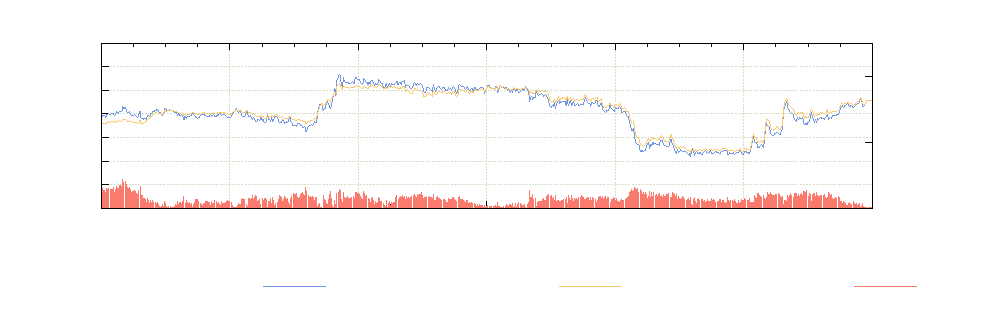
\includegraphics[trim=0 0 0.1cm 0, clip]{Graphs/4/KusVerify/Power/Power}}}%
    \gplfronttext
  \end{picture}%
\endgroup
}
		(b)\\
		\caption{Verification of the total (a) flow and (b) power of the system using the actual pressure profile.}
		\label{fig: Verification Power kusasalethu}
	\end{figure}

	Once all the power and flow parameters were checked calibrated with minimal error, the systems response to the pressure set-points was checked. The compressor models were replaced with the pressure set-point profile instead of the measured outlet pressure profile. The simulated outlet pressure was then compared to the actual measured outlet, this is shown in Figure \ref{fig: Verification Pressure kusasalethu Setpoint}.

	\begin{figure}[h]
		\centering
		\fbox{% GNUPLOT: LaTeX picture with Postscript
\begingroup
  \makeatletter
  \providecommand\color[2][]{%
    \GenericError{(gnuplot) \space\space\space\@spaces}{%
      Package color not loaded in conjunction with
      terminal option `colourtext'%
    }{See the gnuplot documentation for explanation.%
    }{Either use 'blacktext' in gnuplot or load the package
      color.sty in LaTeX.}%
    \renewcommand\color[2][]{}%
  }%
  \providecommand\includegraphics[2][]{%
    \GenericError{(gnuplot) \space\space\space\@spaces}{%
      Package graphicx or graphics not loaded%
    }{See the gnuplot documentation for explanation.%
    }{The gnuplot epslatex terminal needs graphicx.sty or graphics.sty.}%
    \renewcommand\includegraphics[2][]{}%
  }%
  \providecommand\rotatebox[2]{#2}%
  \@ifundefined{ifGPcolor}{%
    \newif\ifGPcolor
    \GPcolortrue
  }{}%
  \@ifundefined{ifGPblacktext}{%
    \newif\ifGPblacktext
    \GPblacktextfalse
  }{}%
  % define a \g@addto@macro without @ in the name:
  \let\gplgaddtomacro\g@addto@macro
  % define empty templates for all commands taking text:
  \gdef\gplbacktext{}%
  \gdef\gplfronttext{}%
  \makeatother
  \ifGPblacktext
    % no textcolor at all
    \def\colorrgb#1{}%
    \def\colorgray#1{}%
  \else
    % gray or color?
    \ifGPcolor
      \def\colorrgb#1{\color[rgb]{#1}}%
      \def\colorgray#1{\color[gray]{#1}}%
      \expandafter\def\csname LTw\endcsname{\color{white}}%
      \expandafter\def\csname LTb\endcsname{\color{black}}%
      \expandafter\def\csname LTa\endcsname{\color{black}}%
      \expandafter\def\csname LT0\endcsname{\color[rgb]{1,0,0}}%
      \expandafter\def\csname LT1\endcsname{\color[rgb]{0,1,0}}%
      \expandafter\def\csname LT2\endcsname{\color[rgb]{0,0,1}}%
      \expandafter\def\csname LT3\endcsname{\color[rgb]{1,0,1}}%
      \expandafter\def\csname LT4\endcsname{\color[rgb]{0,1,1}}%
      \expandafter\def\csname LT5\endcsname{\color[rgb]{1,1,0}}%
      \expandafter\def\csname LT6\endcsname{\color[rgb]{0,0,0}}%
      \expandafter\def\csname LT7\endcsname{\color[rgb]{1,0.3,0}}%
      \expandafter\def\csname LT8\endcsname{\color[rgb]{0.5,0.5,0.5}}%
    \else
      % gray
      \def\colorrgb#1{\color{black}}%
      \def\colorgray#1{\color[gray]{#1}}%
      \expandafter\def\csname LTw\endcsname{\color{white}}%
      \expandafter\def\csname LTb\endcsname{\color{black}}%
      \expandafter\def\csname LTa\endcsname{\color{black}}%
      \expandafter\def\csname LT0\endcsname{\color{black}}%
      \expandafter\def\csname LT1\endcsname{\color{black}}%
      \expandafter\def\csname LT2\endcsname{\color{black}}%
      \expandafter\def\csname LT3\endcsname{\color{black}}%
      \expandafter\def\csname LT4\endcsname{\color{black}}%
      \expandafter\def\csname LT5\endcsname{\color{black}}%
      \expandafter\def\csname LT6\endcsname{\color{black}}%
      \expandafter\def\csname LT7\endcsname{\color{black}}%
      \expandafter\def\csname LT8\endcsname{\color{black}}%
    \fi
  \fi
    \setlength{\unitlength}{0.0500bp}%
    \ifx\gptboxheight\undefined%
      \newlength{\gptboxheight}%
      \newlength{\gptboxwidth}%
      \newsavebox{\gptboxtext}%
    \fi%
    \setlength{\fboxrule}{0.5pt}%
    \setlength{\fboxsep}{1pt}%
\begin{picture}(9360.00,4032.00)%
    \gplgaddtomacro\gplbacktext{%
      \colorrgb{0.00,0.00,0.00}%
      \put(814,1144){\makebox(0,0)[r]{\strut{}$300$}}%
      \colorrgb{0.00,0.00,0.00}%
      \put(814,2018){\makebox(0,0)[r]{\strut{}$350$}}%
      \colorrgb{0.00,0.00,0.00}%
      \put(814,2893){\makebox(0,0)[r]{\strut{}$400$}}%
      \colorrgb{0.00,0.00,0.00}%
      \put(814,3767){\makebox(0,0)[r]{\strut{}$450$}}%
      \colorrgb{0.00,0.00,0.00}%
      \put(946,924){\makebox(0,0){\strut{}00:00}}%
      \colorrgb{0.00,0.00,0.00}%
      \put(2157,924){\makebox(0,0){\strut{}04:00}}%
      \colorrgb{0.00,0.00,0.00}%
      \put(3369,924){\makebox(0,0){\strut{}08:00}}%
      \colorrgb{0.00,0.00,0.00}%
      \put(4580,924){\makebox(0,0){\strut{}12:00}}%
      \colorrgb{0.00,0.00,0.00}%
      \put(5791,924){\makebox(0,0){\strut{}16:00}}%
      \colorrgb{0.00,0.00,0.00}%
      \put(7003,924){\makebox(0,0){\strut{}20:00}}%
      \colorrgb{0.00,0.00,0.00}%
      \put(8214,924){\makebox(0,0){\strut{}00:00}}%
      \colorrgb{0.00,0.00,0.00}%
      \put(8346,1144){\makebox(0,0)[l]{\strut{}$0$}}%
      \colorrgb{0.00,0.00,0.00}%
      \put(8346,2193){\makebox(0,0)[l]{\strut{}$10$}}%
      \colorrgb{0.00,0.00,0.00}%
      \put(8346,3242){\makebox(0,0)[l]{\strut{}$20$}}%
    }%
    \gplgaddtomacro\gplfronttext{%
      \csname LTb\endcsname%
      \put(176,2455){\rotatebox{-270}{\makebox(0,0){\strut{}Pressure $(kPa)$}}}%
      \put(8851,2455){\rotatebox{-270}{\makebox(0,0){\strut{}$\% error$}}}%
      \put(4580,594){\makebox(0,0){\strut{}Time of Day}}%
      \csname LTb\endcsname%
      \put(3725,393){\makebox(0,0)[r]{\strut{}Actual}}%
      \csname LTb\endcsname%
      \put(3725,173){\makebox(0,0)[r]{\strut{}Simulation.}}%
      \csname LTb\endcsname%
      \put(6032,393){\makebox(0,0)[r]{\strut{}Set-point}}%
      \csname LTb\endcsname%
      \put(5900,173){\makebox(0,0)[r]{\strut{}Rel. Error}}%
    }%
    \gplbacktext
    \put(0,0){\fbox{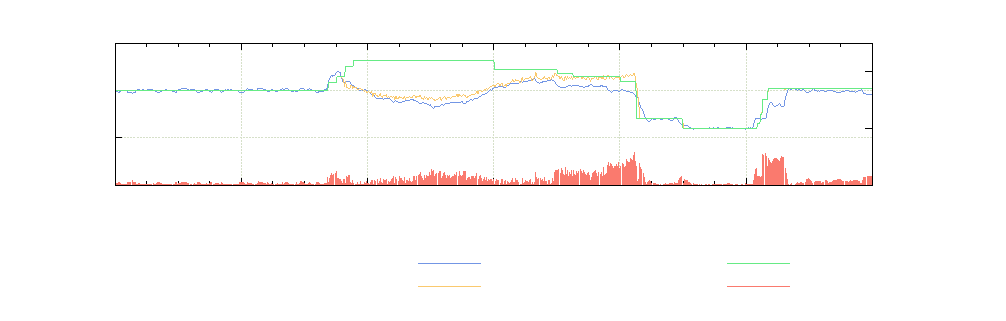
\includegraphics[trim=0 0 0.1cm 0, clip]{Graphs/4/KusVerify/Pressure2/Pressure2}}}%
    \gplfronttext
  \end{picture}%
\endgroup
}
		\caption{Verifying the Pressure response of the system give the pressure set points as inputs}
		\label{fig: Verification Pressure kusasalethu Setpoint}
	\end{figure}
	\par 
	It was noted the during peak air usage periods, between 07:00 and 13:00, that the outlet pressure dropped well below the desired set-point. This was because the compressors struggled to keep up with the air demand during those periods, resulting in a pressure difference as much as 50 kpa from the desired set-point. This was reproduced in the simulation with high accuracy.
	\subsection{Scenario 1. Refuge bay simulation}
	From investigations that were conducted on the mines compressed system, unnecessary refuge bay leaks was identified as a significant inefficiency that can be reduced. Early tests on a single mining level indicated that a reduction refuge bay leaks, by closing the valves would lead to a air saving of $0.05$ $kg/s$ per refuge bay at typical operational pressures. This measurement was conservative as not all of the refuge bays on the level could be closed for the test.
	\par 
	Further tests, integrating more refuge bays for a longer period would not be possible without buy in from the mine's management. To gain this buy-in, the potential financial and operational benefits of refuge bay leakage interventions would first need to be quantified. A simulation model was hence developed to accurately estimate the savings for any interventions.
	\par
	Refuge bay components were added to the baseline modelled discussed previously. Using the test results, refuge bay leaks were added to the simulation model. \gls{scada} data was used to verify the new baseline simulation model with an accuracy of 98\%. Using the per-level layouts obtained from the investigation the location and number of refuge bay components were identified. The full simulation model is shown in Figure \ref{fig: Refuge bay layout} in Appendix \ref{ASchematics}.
	\par 
	
	\begin{figure}[h]
		\centering
		\fbox{% GNUPLOT: LaTeX picture with Postscript
\begingroup
  \makeatletter
  \providecommand\color[2][]{%
    \GenericError{(gnuplot) \space\space\space\@spaces}{%
      Package color not loaded in conjunction with
      terminal option `colourtext'%
    }{See the gnuplot documentation for explanation.%
    }{Either use 'blacktext' in gnuplot or load the package
      color.sty in LaTeX.}%
    \renewcommand\color[2][]{}%
  }%
  \providecommand\includegraphics[2][]{%
    \GenericError{(gnuplot) \space\space\space\@spaces}{%
      Package graphicx or graphics not loaded%
    }{See the gnuplot documentation for explanation.%
    }{The gnuplot epslatex terminal needs graphicx.sty or graphics.sty.}%
    \renewcommand\includegraphics[2][]{}%
  }%
  \providecommand\rotatebox[2]{#2}%
  \@ifundefined{ifGPcolor}{%
    \newif\ifGPcolor
    \GPcolortrue
  }{}%
  \@ifundefined{ifGPblacktext}{%
    \newif\ifGPblacktext
    \GPblacktextfalse
  }{}%
  % define a \g@addto@macro without @ in the name:
  \let\gplgaddtomacro\g@addto@macro
  % define empty templates for all commands taking text:
  \gdef\gplbacktext{}%
  \gdef\gplfronttext{}%
  \makeatother
  \ifGPblacktext
    % no textcolor at all
    \def\colorrgb#1{}%
    \def\colorgray#1{}%
  \else
    % gray or color?
    \ifGPcolor
      \def\colorrgb#1{\color[rgb]{#1}}%
      \def\colorgray#1{\color[gray]{#1}}%
      \expandafter\def\csname LTw\endcsname{\color{white}}%
      \expandafter\def\csname LTb\endcsname{\color{black}}%
      \expandafter\def\csname LTa\endcsname{\color{black}}%
      \expandafter\def\csname LT0\endcsname{\color[rgb]{1,0,0}}%
      \expandafter\def\csname LT1\endcsname{\color[rgb]{0,1,0}}%
      \expandafter\def\csname LT2\endcsname{\color[rgb]{0,0,1}}%
      \expandafter\def\csname LT3\endcsname{\color[rgb]{1,0,1}}%
      \expandafter\def\csname LT4\endcsname{\color[rgb]{0,1,1}}%
      \expandafter\def\csname LT5\endcsname{\color[rgb]{1,1,0}}%
      \expandafter\def\csname LT6\endcsname{\color[rgb]{0,0,0}}%
      \expandafter\def\csname LT7\endcsname{\color[rgb]{1,0.3,0}}%
      \expandafter\def\csname LT8\endcsname{\color[rgb]{0.5,0.5,0.5}}%
    \else
      % gray
      \def\colorrgb#1{\color{black}}%
      \def\colorgray#1{\color[gray]{#1}}%
      \expandafter\def\csname LTw\endcsname{\color{white}}%
      \expandafter\def\csname LTb\endcsname{\color{black}}%
      \expandafter\def\csname LTa\endcsname{\color{black}}%
      \expandafter\def\csname LT0\endcsname{\color{black}}%
      \expandafter\def\csname LT1\endcsname{\color{black}}%
      \expandafter\def\csname LT2\endcsname{\color{black}}%
      \expandafter\def\csname LT3\endcsname{\color{black}}%
      \expandafter\def\csname LT4\endcsname{\color{black}}%
      \expandafter\def\csname LT5\endcsname{\color{black}}%
      \expandafter\def\csname LT6\endcsname{\color{black}}%
      \expandafter\def\csname LT7\endcsname{\color{black}}%
      \expandafter\def\csname LT8\endcsname{\color{black}}%
    \fi
  \fi
    \setlength{\unitlength}{0.0500bp}%
    \ifx\gptboxheight\undefined%
      \newlength{\gptboxheight}%
      \newlength{\gptboxwidth}%
      \newsavebox{\gptboxtext}%
    \fi%
    \setlength{\fboxrule}{0.5pt}%
    \setlength{\fboxsep}{1pt}%
\begin{picture}(9360.00,3780.00)%
    \gplgaddtomacro\gplbacktext{%
      \colorrgb{0.00,0.00,0.00}%
      \put(682,924){\makebox(0,0)[r]{\strut{}$0$}}%
      \colorrgb{0.00,0.00,0.00}%
      \put(682,1788){\makebox(0,0)[r]{\strut{}$5$}}%
      \colorrgb{0.00,0.00,0.00}%
      \put(682,2651){\makebox(0,0)[r]{\strut{}$10$}}%
      \colorrgb{0.00,0.00,0.00}%
      \put(682,3515){\makebox(0,0)[r]{\strut{}$15$}}%
      \colorrgb{0.00,0.00,0.00}%
      \put(814,704){\makebox(0,0){\strut{}00:00}}%
      \colorrgb{0.00,0.00,0.00}%
      \put(2172,704){\makebox(0,0){\strut{}04:00}}%
      \colorrgb{0.00,0.00,0.00}%
      \put(3530,704){\makebox(0,0){\strut{}08:00}}%
      \colorrgb{0.00,0.00,0.00}%
      \put(4888,704){\makebox(0,0){\strut{}12:00}}%
      \colorrgb{0.00,0.00,0.00}%
      \put(6246,704){\makebox(0,0){\strut{}16:00}}%
      \colorrgb{0.00,0.00,0.00}%
      \put(7604,704){\makebox(0,0){\strut{}20:00}}%
      \colorrgb{0.00,0.00,0.00}%
      \put(8962,704){\makebox(0,0){\strut{}00:00}}%
    }%
    \gplgaddtomacro\gplfronttext{%
      \csname LTb\endcsname%
      \put(176,2219){\rotatebox{-270}{\makebox(0,0){\strut{}Power $(MW)$}}}%
      \put(4888,374){\makebox(0,0){\strut{}Time of Day}}%
      \csname LTb\endcsname%
      \put(2813,173){\makebox(0,0)[r]{\strut{}Baseline}}%
      \csname LTb\endcsname%
      \put(5252,173){\makebox(0,0)[r]{\strut{}Intervention}}%
      \csname LTb\endcsname%
      \put(7691,173){\makebox(0,0)[r]{\strut{}Power saving}}%
    }%
    \gplbacktext
    \put(0,0){
\includegraphics{Graphs/4/KUSResults/RefugePower/RefugePower}}%
    \gplfronttext
  \end{picture}%
\endgroup
}
		\caption{The Baseline system power compared to the system power when refuge bay leaks are reduce.}
		\label{fig: RefugeBay Power.}
	\end{figure}   

	\begin{figure}[h]
		\centering
		\fbox{% GNUPLOT: LaTeX picture with Postscript
\begingroup
  \makeatletter
  \providecommand\color[2][]{%
    \GenericError{(gnuplot) \space\space\space\@spaces}{%
      Package color not loaded in conjunction with
      terminal option `colourtext'%
    }{See the gnuplot documentation for explanation.%
    }{Either use 'blacktext' in gnuplot or load the package
      color.sty in LaTeX.}%
    \renewcommand\color[2][]{}%
  }%
  \providecommand\includegraphics[2][]{%
    \GenericError{(gnuplot) \space\space\space\@spaces}{%
      Package graphicx or graphics not loaded%
    }{See the gnuplot documentation for explanation.%
    }{The gnuplot epslatex terminal needs graphicx.sty or graphics.sty.}%
    \renewcommand\includegraphics[2][]{}%
  }%
  \providecommand\rotatebox[2]{#2}%
  \@ifundefined{ifGPcolor}{%
    \newif\ifGPcolor
    \GPcolortrue
  }{}%
  \@ifundefined{ifGPblacktext}{%
    \newif\ifGPblacktext
    \GPblacktextfalse
  }{}%
  % define a \g@addto@macro without @ in the name:
  \let\gplgaddtomacro\g@addto@macro
  % define empty templates for all commands taking text:
  \gdef\gplbacktext{}%
  \gdef\gplfronttext{}%
  \makeatother
  \ifGPblacktext
    % no textcolor at all
    \def\colorrgb#1{}%
    \def\colorgray#1{}%
  \else
    % gray or color?
    \ifGPcolor
      \def\colorrgb#1{\color[rgb]{#1}}%
      \def\colorgray#1{\color[gray]{#1}}%
      \expandafter\def\csname LTw\endcsname{\color{white}}%
      \expandafter\def\csname LTb\endcsname{\color{black}}%
      \expandafter\def\csname LTa\endcsname{\color{black}}%
      \expandafter\def\csname LT0\endcsname{\color[rgb]{1,0,0}}%
      \expandafter\def\csname LT1\endcsname{\color[rgb]{0,1,0}}%
      \expandafter\def\csname LT2\endcsname{\color[rgb]{0,0,1}}%
      \expandafter\def\csname LT3\endcsname{\color[rgb]{1,0,1}}%
      \expandafter\def\csname LT4\endcsname{\color[rgb]{0,1,1}}%
      \expandafter\def\csname LT5\endcsname{\color[rgb]{1,1,0}}%
      \expandafter\def\csname LT6\endcsname{\color[rgb]{0,0,0}}%
      \expandafter\def\csname LT7\endcsname{\color[rgb]{1,0.3,0}}%
      \expandafter\def\csname LT8\endcsname{\color[rgb]{0.5,0.5,0.5}}%
    \else
      % gray
      \def\colorrgb#1{\color{black}}%
      \def\colorgray#1{\color[gray]{#1}}%
      \expandafter\def\csname LTw\endcsname{\color{white}}%
      \expandafter\def\csname LTb\endcsname{\color{black}}%
      \expandafter\def\csname LTa\endcsname{\color{black}}%
      \expandafter\def\csname LT0\endcsname{\color{black}}%
      \expandafter\def\csname LT1\endcsname{\color{black}}%
      \expandafter\def\csname LT2\endcsname{\color{black}}%
      \expandafter\def\csname LT3\endcsname{\color{black}}%
      \expandafter\def\csname LT4\endcsname{\color{black}}%
      \expandafter\def\csname LT5\endcsname{\color{black}}%
      \expandafter\def\csname LT6\endcsname{\color{black}}%
      \expandafter\def\csname LT7\endcsname{\color{black}}%
      \expandafter\def\csname LT8\endcsname{\color{black}}%
    \fi
  \fi
    \setlength{\unitlength}{0.0500bp}%
    \ifx\gptboxheight\undefined%
      \newlength{\gptboxheight}%
      \newlength{\gptboxwidth}%
      \newsavebox{\gptboxtext}%
    \fi%
    \setlength{\fboxrule}{0.5pt}%
    \setlength{\fboxsep}{1pt}%
\begin{picture}(9360.00,3780.00)%
    \gplgaddtomacro\gplbacktext{%
      \colorrgb{0.00,0.00,0.00}%
      \put(814,1183){\makebox(0,0)[r]{\strut{}$360$}}%
      \colorrgb{0.00,0.00,0.00}%
      \put(814,1701){\makebox(0,0)[r]{\strut{}$380$}}%
      \colorrgb{0.00,0.00,0.00}%
      \put(814,2220){\makebox(0,0)[r]{\strut{}$400$}}%
      \colorrgb{0.00,0.00,0.00}%
      \put(814,2738){\makebox(0,0)[r]{\strut{}$420$}}%
      \colorrgb{0.00,0.00,0.00}%
      \put(814,3256){\makebox(0,0)[r]{\strut{}$440$}}%
      \colorrgb{0.00,0.00,0.00}%
      \put(946,704){\makebox(0,0){\strut{}00:00}}%
      \colorrgb{0.00,0.00,0.00}%
      \put(2282,704){\makebox(0,0){\strut{}04:00}}%
      \colorrgb{0.00,0.00,0.00}%
      \put(3618,704){\makebox(0,0){\strut{}08:00}}%
      \colorrgb{0.00,0.00,0.00}%
      \put(4954,704){\makebox(0,0){\strut{}12:00}}%
      \colorrgb{0.00,0.00,0.00}%
      \put(6290,704){\makebox(0,0){\strut{}16:00}}%
      \colorrgb{0.00,0.00,0.00}%
      \put(7626,704){\makebox(0,0){\strut{}20:00}}%
      \colorrgb{0.00,0.00,0.00}%
      \put(8962,704){\makebox(0,0){\strut{}00:00}}%
    }%
    \gplgaddtomacro\gplfronttext{%
      \csname LTb\endcsname%
      \put(176,2219){\rotatebox{-270}{\makebox(0,0){\strut{}Pressure $(kPa)$}}}%
      \put(4954,374){\makebox(0,0){\strut{}Time of Day}}%
      \csname LTb\endcsname%
      \put(4099,173){\makebox(0,0)[r]{\strut{}Baseline}}%
      \csname LTb\endcsname%
      \put(6538,173){\makebox(0,0)[r]{\strut{}Intervention}}%
    }%
    \gplbacktext
    \put(0,0){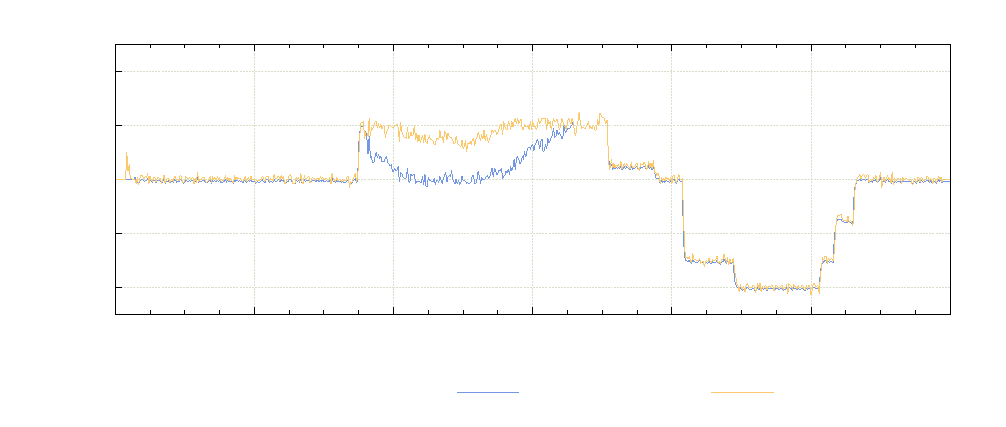
\includegraphics{Graphs/4/KUSResults/RefugePressure/RefugePressure}}%
    \gplfronttext
  \end{picture}%
\endgroup
}
		\caption{The Baseline system pressure compared to the system pressure when refuge bay leaks are reduce.}
		\label{fig: RefugeBay Pressures.}
	\end{figure}  
	Tested scenario where all excessive leaking valves are removed.
	Refuge bays savings 1MW E.E.
	
	\subsection{Scenario 2. Closing off levels/stopes}
	The effect of in-stope control during peak times was simulated for 105L. The level was modelled to include all major leaks, refuge bays and drilling sections that were manually identified. For comparison, station isolation and the combination of in-stope control and station isolation were simulated. 
	
	
	\subsection{Validation of results}
	
	- awaiting results on manual tests
	
	\subsection{Summary}
\newpage
\section{Periodic simulation analysis}
	\subsection{Preamble}
	Updating the inputs of a simulation periodically could be used to verify simulation model accuracy. Simulation outputs remaining precise for subsequent days would indicate that the model is correctly calibrated. Additionally, periodic simulation could be used to identify significant operational changes that occur within the actual system. This would cause the simulation outputs to differ from the actual measured parameters. 
	\par 
	Periodic simulation was implemented using the process shown in Figure \ref{fig: PeriodicProcess}. Simulation input data is collected for the simulation period, this data includes only inputs that vary day to day such as schedules, ambient air conditions and  measured flows. Once the input values are collected, they are then imported into the compressed air model. The simulation performed and the output data is exported. An analysis is then performed to compare the simulated period with the actual operation of the system. This process is then repeated periodically.
		\begin{figure}[h]
		\centering
		\fbox{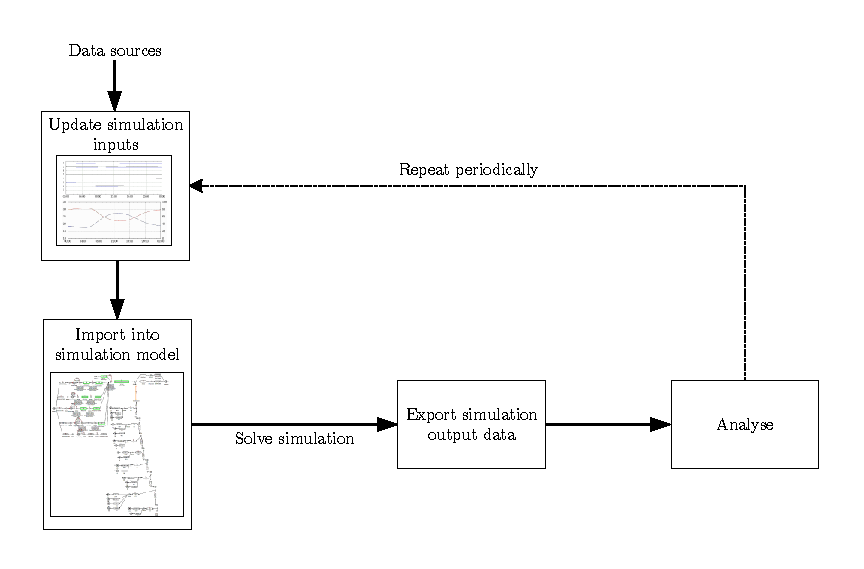
\includegraphics[trim =0cm 0.5cm 0cm 1cm,width=\textwidth]{Graphs/4/PeriodicProcess/PeriodicProcess.pdf}}
		\caption{The periodic simulation process that was followed in this analysis.}
		\label{fig: PeriodicProcess}
	\end{figure}	
	     \subsection{Results}
	     Daily periodic simulation was implemented between 2016/11/01 and 2016/11/30. For each period, the simulated total flow, shaft delivery pressure and total power consumption were compared to the actual operation. The results of this analysis are shown in Figure \ref{fig: Periodic simulation}.
	     \par 
	     
	\begin{figure}[h]
		\centering
		\fbox{% GNUPLOT: LaTeX picture with Postscript
\begingroup
  \makeatletter
  \providecommand\color[2][]{%
    \GenericError{(gnuplot) \space\space\space\@spaces}{%
      Package color not loaded in conjunction with
      terminal option `colourtext'%
    }{See the gnuplot documentation for explanation.%
    }{Either use 'blacktext' in gnuplot or load the package
      color.sty in LaTeX.}%
    \renewcommand\color[2][]{}%
  }%
  \providecommand\includegraphics[2][]{%
    \GenericError{(gnuplot) \space\space\space\@spaces}{%
      Package graphicx or graphics not loaded%
    }{See the gnuplot documentation for explanation.%
    }{The gnuplot epslatex terminal needs graphicx.sty or graphics.sty.}%
    \renewcommand\includegraphics[2][]{}%
  }%
  \providecommand\rotatebox[2]{#2}%
  \@ifundefined{ifGPcolor}{%
    \newif\ifGPcolor
    \GPcolortrue
  }{}%
  \@ifundefined{ifGPblacktext}{%
    \newif\ifGPblacktext
    \GPblacktextfalse
  }{}%
  % define a \g@addto@macro without @ in the name:
  \let\gplgaddtomacro\g@addto@macro
  % define empty templates for all commands taking text:
  \gdef\gplbacktext{}%
  \gdef\gplfronttext{}%
  \makeatother
  \ifGPblacktext
    % no textcolor at all
    \def\colorrgb#1{}%
    \def\colorgray#1{}%
  \else
    % gray or color?
    \ifGPcolor
      \def\colorrgb#1{\color[rgb]{#1}}%
      \def\colorgray#1{\color[gray]{#1}}%
      \expandafter\def\csname LTw\endcsname{\color{white}}%
      \expandafter\def\csname LTb\endcsname{\color{black}}%
      \expandafter\def\csname LTa\endcsname{\color{black}}%
      \expandafter\def\csname LT0\endcsname{\color[rgb]{1,0,0}}%
      \expandafter\def\csname LT1\endcsname{\color[rgb]{0,1,0}}%
      \expandafter\def\csname LT2\endcsname{\color[rgb]{0,0,1}}%
      \expandafter\def\csname LT3\endcsname{\color[rgb]{1,0,1}}%
      \expandafter\def\csname LT4\endcsname{\color[rgb]{0,1,1}}%
      \expandafter\def\csname LT5\endcsname{\color[rgb]{1,1,0}}%
      \expandafter\def\csname LT6\endcsname{\color[rgb]{0,0,0}}%
      \expandafter\def\csname LT7\endcsname{\color[rgb]{1,0.3,0}}%
      \expandafter\def\csname LT8\endcsname{\color[rgb]{0.5,0.5,0.5}}%
    \else
      % gray
      \def\colorrgb#1{\color{black}}%
      \def\colorgray#1{\color[gray]{#1}}%
      \expandafter\def\csname LTw\endcsname{\color{white}}%
      \expandafter\def\csname LTb\endcsname{\color{black}}%
      \expandafter\def\csname LTa\endcsname{\color{black}}%
      \expandafter\def\csname LT0\endcsname{\color{black}}%
      \expandafter\def\csname LT1\endcsname{\color{black}}%
      \expandafter\def\csname LT2\endcsname{\color{black}}%
      \expandafter\def\csname LT3\endcsname{\color{black}}%
      \expandafter\def\csname LT4\endcsname{\color{black}}%
      \expandafter\def\csname LT5\endcsname{\color{black}}%
      \expandafter\def\csname LT6\endcsname{\color{black}}%
      \expandafter\def\csname LT7\endcsname{\color{black}}%
      \expandafter\def\csname LT8\endcsname{\color{black}}%
    \fi
  \fi
    \setlength{\unitlength}{0.0500bp}%
    \ifx\gptboxheight\undefined%
      \newlength{\gptboxheight}%
      \newlength{\gptboxwidth}%
      \newsavebox{\gptboxtext}%
    \fi%
    \setlength{\fboxrule}{0.5pt}%
    \setlength{\fboxsep}{1pt}%
\begin{picture}(9360.00,4032.00)%
    \gplgaddtomacro\gplbacktext{%
      \colorrgb{0.00,0.00,0.00}%
      \put(814,924){\makebox(0,0)[r]{\strut{}$80$}}%
      \colorrgb{0.00,0.00,0.00}%
      \put(814,1635){\makebox(0,0)[r]{\strut{}$85$}}%
      \colorrgb{0.00,0.00,0.00}%
      \put(814,2346){\makebox(0,0)[r]{\strut{}$90$}}%
      \colorrgb{0.00,0.00,0.00}%
      \put(814,3056){\makebox(0,0)[r]{\strut{}$95$}}%
      \colorrgb{0.00,0.00,0.00}%
      \put(814,3767){\makebox(0,0)[r]{\strut{}$100$}}%
      \colorrgb{0.00,0.00,0.00}%
      \put(946,704){\makebox(0,0){\strut{}2016/11/01}}%
      \colorrgb{0.00,0.00,0.00}%
      \put(2604,704){\makebox(0,0){\strut{}2016/11/07}}%
      \colorrgb{0.00,0.00,0.00}%
      \put(4263,704){\makebox(0,0){\strut{}2016/11/13}}%
      \colorrgb{0.00,0.00,0.00}%
      \put(5921,704){\makebox(0,0){\strut{}2016/11/19}}%
      \colorrgb{0.00,0.00,0.00}%
      \put(7580,704){\makebox(0,0){\strut{}2016/11/25}}%
    }%
    \gplgaddtomacro\gplfronttext{%
      \csname LTb\endcsname%
      \put(176,2345){\rotatebox{-270}{\makebox(0,0){\strut{}Accuracy (\%)}}}%
      \put(4954,374){\makebox(0,0){\strut{}Date of simulation}}%
      \csname LTb\endcsname%
      \put(3143,173){\makebox(0,0)[r]{\strut{}Flow}}%
      \csname LTb\endcsname%
      \put(5054,173){\makebox(0,0)[r]{\strut{}Pressure}}%
      \csname LTb\endcsname%
      \put(6965,173){\makebox(0,0)[r]{\strut{}Power}}%
    }%
    \gplbacktext
    \put(0,0){\fbox{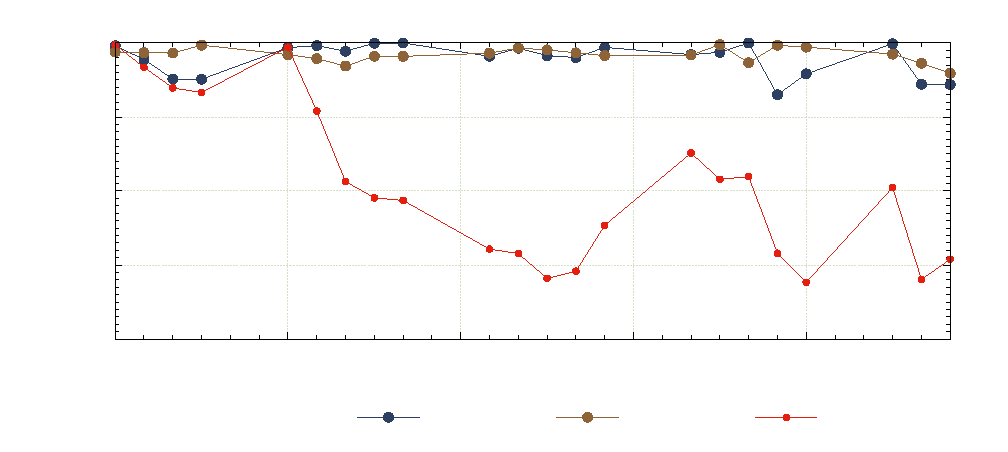
\includegraphics[trim=0 0 0.1cm 0, clip]{Graphs/4/Periodic1/Periodic1}}}%
    \gplfronttext
  \end{picture}%
\endgroup
}
		\caption{The flow, pressure and power error percentages for daily periodic simulations over a month.}
		\label{fig: Periodic simulation}
	\end{figure}   
The accuracy of the flow and pressure parameters of the model remained precise for the duration of the periodic simulation. However From the 2016/11/07, the accuracy of the simulated power dropped by between 10 and 15 percent. The daily average power of the system up to the point was approximately 12.5 MW, a 15\% simulation error therefore relates to 1.9 MW. This suggests a major shift in operation of the system.
\par 
A deeper analysis was to try ascertain the source of the operational change. From analysis it was noticed that the simulated power for compressor 1  no longer reflected the actual measurements. A look at the actual power measurement for compressor 1 showed a sharp decline in power starting from the 2016/11/07. At the same time the efficiency, or amount of power required per kg/s of air, of the system increased significantly from the same date. This is shown in Figure \ref{fig: MeasurementAccuracy.}. The results that there was either a major change on compressor 1 that increased the efficiency or their was a malfunction with the power meter.
	\begin{figure}[h]
		\centering
		\fbox{% GNUPLOT: LaTeX picture with Postscript
\begingroup
  \makeatletter
  \providecommand\color[2][]{%
    \GenericError{(gnuplot) \space\space\space\@spaces}{%
      Package color not loaded in conjunction with
      terminal option `colourtext'%
    }{See the gnuplot documentation for explanation.%
    }{Either use 'blacktext' in gnuplot or load the package
      color.sty in LaTeX.}%
    \renewcommand\color[2][]{}%
  }%
  \providecommand\includegraphics[2][]{%
    \GenericError{(gnuplot) \space\space\space\@spaces}{%
      Package graphicx or graphics not loaded%
    }{See the gnuplot documentation for explanation.%
    }{The gnuplot epslatex terminal needs graphicx.sty or graphics.sty.}%
    \renewcommand\includegraphics[2][]{}%
  }%
  \providecommand\rotatebox[2]{#2}%
  \@ifundefined{ifGPcolor}{%
    \newif\ifGPcolor
    \GPcolortrue
  }{}%
  \@ifundefined{ifGPblacktext}{%
    \newif\ifGPblacktext
    \GPblacktextfalse
  }{}%
  % define a \g@addto@macro without @ in the name:
  \let\gplgaddtomacro\g@addto@macro
  % define empty templates for all commands taking text:
  \gdef\gplbacktext{}%
  \gdef\gplfronttext{}%
  \makeatother
  \ifGPblacktext
    % no textcolor at all
    \def\colorrgb#1{}%
    \def\colorgray#1{}%
  \else
    % gray or color?
    \ifGPcolor
      \def\colorrgb#1{\color[rgb]{#1}}%
      \def\colorgray#1{\color[gray]{#1}}%
      \expandafter\def\csname LTw\endcsname{\color{white}}%
      \expandafter\def\csname LTb\endcsname{\color{black}}%
      \expandafter\def\csname LTa\endcsname{\color{black}}%
      \expandafter\def\csname LT0\endcsname{\color[rgb]{1,0,0}}%
      \expandafter\def\csname LT1\endcsname{\color[rgb]{0,1,0}}%
      \expandafter\def\csname LT2\endcsname{\color[rgb]{0,0,1}}%
      \expandafter\def\csname LT3\endcsname{\color[rgb]{1,0,1}}%
      \expandafter\def\csname LT4\endcsname{\color[rgb]{0,1,1}}%
      \expandafter\def\csname LT5\endcsname{\color[rgb]{1,1,0}}%
      \expandafter\def\csname LT6\endcsname{\color[rgb]{0,0,0}}%
      \expandafter\def\csname LT7\endcsname{\color[rgb]{1,0.3,0}}%
      \expandafter\def\csname LT8\endcsname{\color[rgb]{0.5,0.5,0.5}}%
    \else
      % gray
      \def\colorrgb#1{\color{black}}%
      \def\colorgray#1{\color[gray]{#1}}%
      \expandafter\def\csname LTw\endcsname{\color{white}}%
      \expandafter\def\csname LTb\endcsname{\color{black}}%
      \expandafter\def\csname LTa\endcsname{\color{black}}%
      \expandafter\def\csname LT0\endcsname{\color{black}}%
      \expandafter\def\csname LT1\endcsname{\color{black}}%
      \expandafter\def\csname LT2\endcsname{\color{black}}%
      \expandafter\def\csname LT3\endcsname{\color{black}}%
      \expandafter\def\csname LT4\endcsname{\color{black}}%
      \expandafter\def\csname LT5\endcsname{\color{black}}%
      \expandafter\def\csname LT6\endcsname{\color{black}}%
      \expandafter\def\csname LT7\endcsname{\color{black}}%
      \expandafter\def\csname LT8\endcsname{\color{black}}%
    \fi
  \fi
    \setlength{\unitlength}{0.0500bp}%
    \ifx\gptboxheight\undefined%
      \newlength{\gptboxheight}%
      \newlength{\gptboxwidth}%
      \newsavebox{\gptboxtext}%
    \fi%
    \setlength{\fboxrule}{0.5pt}%
    \setlength{\fboxsep}{1pt}%
\begin{picture}(9360.00,3528.00)%
    \gplgaddtomacro\gplbacktext{%
      \colorrgb{0.00,0.00,0.00}%
      \put(946,924){\makebox(0,0)[r]{\strut{}$1000$}}%
      \colorrgb{0.00,0.00,0.00}%
      \put(946,1314){\makebox(0,0)[r]{\strut{}$1500$}}%
      \colorrgb{0.00,0.00,0.00}%
      \put(946,1704){\makebox(0,0)[r]{\strut{}$2000$}}%
      \colorrgb{0.00,0.00,0.00}%
      \put(946,2094){\makebox(0,0)[r]{\strut{}$2500$}}%
      \colorrgb{0.00,0.00,0.00}%
      \put(946,2483){\makebox(0,0)[r]{\strut{}$3000$}}%
      \colorrgb{0.00,0.00,0.00}%
      \put(946,2873){\makebox(0,0)[r]{\strut{}$3500$}}%
      \colorrgb{0.00,0.00,0.00}%
      \put(946,3263){\makebox(0,0)[r]{\strut{}$4000$}}%
      \colorrgb{0.00,0.00,0.00}%
      \put(1078,704){\makebox(0,0){\strut{}2016/09/01}}%
      \colorrgb{0.00,0.00,0.00}%
      \put(3118,704){\makebox(0,0){\strut{}2016/10/01}}%
      \colorrgb{0.00,0.00,0.00}%
      \put(5226,704){\makebox(0,0){\strut{}2016/11/01}}%
      \colorrgb{0.00,0.00,0.00}%
      \put(5226,704){\makebox(0,0){\strut{}2016/11/01}}%
      \colorrgb{0.00,0.00,0.00}%
      \put(7266,704){\makebox(0,0){\strut{}2016/12/01}}%
      \colorrgb{0.00,0.00,0.00}%
      \put(8214,924){\makebox(0,0)[l]{\strut{}$2$}}%
      \colorrgb{0.00,0.00,0.00}%
      \put(8214,1314){\makebox(0,0)[l]{\strut{}$2.5$}}%
      \colorrgb{0.00,0.00,0.00}%
      \put(8214,1704){\makebox(0,0)[l]{\strut{}$3$}}%
      \colorrgb{0.00,0.00,0.00}%
      \put(8214,2094){\makebox(0,0)[l]{\strut{}$3.5$}}%
      \colorrgb{0.00,0.00,0.00}%
      \put(8214,2483){\makebox(0,0)[l]{\strut{}$4$}}%
      \colorrgb{0.00,0.00,0.00}%
      \put(8214,2873){\makebox(0,0)[l]{\strut{}$4.5$}}%
      \colorrgb{0.00,0.00,0.00}%
      \put(8214,3263){\makebox(0,0)[l]{\strut{}$5$}}%
    }%
    \gplgaddtomacro\gplfronttext{%
      \csname LTb\endcsname%
      \put(176,2093){\rotatebox{-270}{\makebox(0,0){\strut{}Power (kW)}}}%
      \put(8851,2093){\rotatebox{-270}{\makebox(0,0){\strut{}$Flow per Watt (kg/s/W)$}}}%
      \put(4580,374){\makebox(0,0){\strut{}Date}}%
      \csname LTb\endcsname%
      \put(3725,173){\makebox(0,0)[r]{\strut{}Compressor 1 average power}}%
      \csname LTb\endcsname%
      \put(8012,173){\makebox(0,0)[r]{\strut{}System efficiency}}%
      \csname LTb\endcsname%
      \put(6220,3029){\makebox(0,0){\strut{}\shortstack{\small{Periodic simulation}}}}%
    }%
    \gplbacktext
    \put(0,0){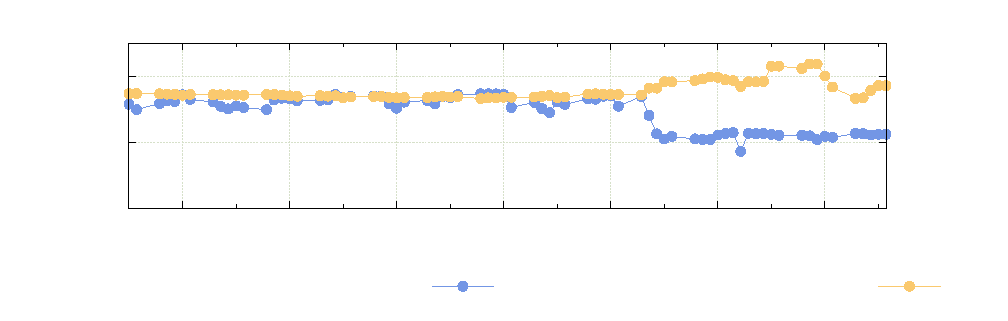
\includegraphics{Graphs/4/PeriodicRange/PeriodicRange}}%
    \gplfronttext
  \end{picture}%
\endgroup
}
		\caption{Supply efficiency and Compressor 1's average power output over the time of the periodic analysis.}
		\label{fig: MeasurementAccuracy.}
	\end{figure}    
	\begin{figure}[h]
		\centering
		\fbox{% GNUPLOT: LaTeX picture with Postscript
\begingroup
  \makeatletter
  \providecommand\color[2][]{%
    \GenericError{(gnuplot) \space\space\space\@spaces}{%
      Package color not loaded in conjunction with
      terminal option `colourtext'%
    }{See the gnuplot documentation for explanation.%
    }{Either use 'blacktext' in gnuplot or load the package
      color.sty in LaTeX.}%
    \renewcommand\color[2][]{}%
  }%
  \providecommand\includegraphics[2][]{%
    \GenericError{(gnuplot) \space\space\space\@spaces}{%
      Package graphicx or graphics not loaded%
    }{See the gnuplot documentation for explanation.%
    }{The gnuplot epslatex terminal needs graphicx.sty or graphics.sty.}%
    \renewcommand\includegraphics[2][]{}%
  }%
  \providecommand\rotatebox[2]{#2}%
  \@ifundefined{ifGPcolor}{%
    \newif\ifGPcolor
    \GPcolortrue
  }{}%
  \@ifundefined{ifGPblacktext}{%
    \newif\ifGPblacktext
    \GPblacktextfalse
  }{}%
  % define a \g@addto@macro without @ in the name:
  \let\gplgaddtomacro\g@addto@macro
  % define empty templates for all commands taking text:
  \gdef\gplbacktext{}%
  \gdef\gplfronttext{}%
  \makeatother
  \ifGPblacktext
    % no textcolor at all
    \def\colorrgb#1{}%
    \def\colorgray#1{}%
  \else
    % gray or color?
    \ifGPcolor
      \def\colorrgb#1{\color[rgb]{#1}}%
      \def\colorgray#1{\color[gray]{#1}}%
      \expandafter\def\csname LTw\endcsname{\color{white}}%
      \expandafter\def\csname LTb\endcsname{\color{black}}%
      \expandafter\def\csname LTa\endcsname{\color{black}}%
      \expandafter\def\csname LT0\endcsname{\color[rgb]{1,0,0}}%
      \expandafter\def\csname LT1\endcsname{\color[rgb]{0,1,0}}%
      \expandafter\def\csname LT2\endcsname{\color[rgb]{0,0,1}}%
      \expandafter\def\csname LT3\endcsname{\color[rgb]{1,0,1}}%
      \expandafter\def\csname LT4\endcsname{\color[rgb]{0,1,1}}%
      \expandafter\def\csname LT5\endcsname{\color[rgb]{1,1,0}}%
      \expandafter\def\csname LT6\endcsname{\color[rgb]{0,0,0}}%
      \expandafter\def\csname LT7\endcsname{\color[rgb]{1,0.3,0}}%
      \expandafter\def\csname LT8\endcsname{\color[rgb]{0.5,0.5,0.5}}%
    \else
      % gray
      \def\colorrgb#1{\color{black}}%
      \def\colorgray#1{\color[gray]{#1}}%
      \expandafter\def\csname LTw\endcsname{\color{white}}%
      \expandafter\def\csname LTb\endcsname{\color{black}}%
      \expandafter\def\csname LTa\endcsname{\color{black}}%
      \expandafter\def\csname LT0\endcsname{\color{black}}%
      \expandafter\def\csname LT1\endcsname{\color{black}}%
      \expandafter\def\csname LT2\endcsname{\color{black}}%
      \expandafter\def\csname LT3\endcsname{\color{black}}%
      \expandafter\def\csname LT4\endcsname{\color{black}}%
      \expandafter\def\csname LT5\endcsname{\color{black}}%
      \expandafter\def\csname LT6\endcsname{\color{black}}%
      \expandafter\def\csname LT7\endcsname{\color{black}}%
      \expandafter\def\csname LT8\endcsname{\color{black}}%
    \fi
  \fi
    \setlength{\unitlength}{0.0500bp}%
    \ifx\gptboxheight\undefined%
      \newlength{\gptboxheight}%
      \newlength{\gptboxwidth}%
      \newsavebox{\gptboxtext}%
    \fi%
    \setlength{\fboxrule}{0.5pt}%
    \setlength{\fboxsep}{1pt}%
\begin{picture}(9360.00,2772.00)%
    \gplgaddtomacro\gplbacktext{%
      \colorrgb{0.00,0.00,0.00}%
      \put(682,924){\makebox(0,0)[r]{\strut{}$0$}}%
      \colorrgb{0.00,0.00,0.00}%
      \put(682,1241){\makebox(0,0)[r]{\strut{}$5$}}%
      \colorrgb{0.00,0.00,0.00}%
      \put(682,1557){\makebox(0,0)[r]{\strut{}$10$}}%
      \colorrgb{0.00,0.00,0.00}%
      \put(682,1874){\makebox(0,0)[r]{\strut{}$15$}}%
      \colorrgb{0.00,0.00,0.00}%
      \put(682,2190){\makebox(0,0)[r]{\strut{}$20$}}%
      \colorrgb{0.00,0.00,0.00}%
      \put(682,2507){\makebox(0,0)[r]{\strut{}$25$}}%
      \colorrgb{0.00,0.00,0.00}%
      \put(1376,704){\makebox(0,0){\strut{}03/11/2016}}%
      \colorrgb{0.00,0.00,0.00}%
      \put(3343,704){\makebox(0,0){\strut{}10/11/2016}}%
      \colorrgb{0.00,0.00,0.00}%
      \put(5309,704){\makebox(0,0){\strut{}17/11/2016}}%
      \colorrgb{0.00,0.00,0.00}%
      \put(7276,704){\makebox(0,0){\strut{}24/11/2016}}%
    }%
    \gplgaddtomacro\gplfronttext{%
      \csname LTb\endcsname%
      \put(176,1715){\rotatebox{-270}{\makebox(0,0){\strut{}Error \%}}}%
      \put(4888,374){\makebox(0,0){\strut{}Date of simulation}}%
      \csname LTb\endcsname%
      \put(3077,173){\makebox(0,0)[r]{\strut{}Flow}}%
      \csname LTb\endcsname%
      \put(4988,173){\makebox(0,0)[r]{\strut{}Pressure}}%
      \csname LTb\endcsname%
      \put(6899,173){\makebox(0,0)[r]{\strut{}Power}}%
    }%
    \gplbacktext
    \put(0,0){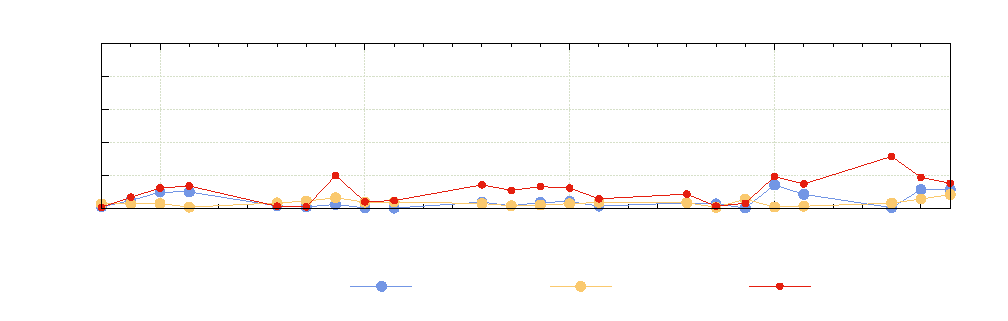
\includegraphics{Graphs/4/Periodic2/Periodic2}}%
    \gplfronttext
  \end{picture}%
\endgroup
}
		\caption{Corrected periodic.}
		\label{fig: Corrected Periodic simulation}
	\end{figure}    
	\subsection{Validation}
	\subsection{Summary}
\newpage
\section{Potential benefit for SA mines}

	Using  
\section{Conclusion}